
% This is a simple template for a LaTeX document using the "article" class.
% See "book", "report", "letter" for other types of document.

\documentclass[10pt]{article} % use larger type; default would be 10pt

\usepackage[T1]{fontenc}
\usepackage[french]{babel}
\usepackage[utf8]{inputenc} % set input encoding (not needed with XeLaTeX)
\usepackage{kpfonts}
\usepackage{hyperref}
\usepackage{listings}

%%% Examples of Article customizations
% These packages are optional, depending whether you want the features they provide.
% See the LaTeX Companion or other references for full information.

%%% PAGE DIMENSIONS
\usepackage{geometry} % to change the page dimensions
\geometry{a4paper} % or letterpaper (US) or a5paper or....
% THE MARGINS FOR DSA is 1.5cm
\geometry{margin=1.5cm} % for example, change the margins to 2 inches all round
% \geometry{landscape} % set up the page for landscape
%   read geometry.pdf for detailed page layout information


% \usepackage[parfill]{parskip} % Activate to begin paragraphs with an empty line rather than an indent

%%% PACKAGES
\usepackage{booktabs} % for much better looking tables
\usepackage{array} % for better arrays (eg matrices) in maths
\usepackage{paralist} % very flexible & customisable lists (eg. enumerate/itemize, etc.)
\usepackage{verbatim} % adds environment for commenting out blocks of text & for better verbatim
% \usepackage{subfig} % make it possible to include more than one captioned figure/table in a single float
% These packages are all incorporated in the memoir class to one degree or another...

%%% HEADERS & FOOTERS
\usepackage{fancyhdr} % This should be set AFTER setting up the page geometry
% \pagestyle{fancy} % options: empty , plain , fancy

\usepackage{graphicx} % support the \includegraphics command and options
\usepackage{subcaption}
\usepackage{caption}

\usepackage{dingbat} % For the pointy hands
\usepackage{pifont}
% \usepackage{xcolor} % For pretty colors
\usepackage[table]{xcolor}
\usepackage{tikz} % for nice pictures
\usepackage{blindtext}
\usepackage{wrapfig}
\usepackage{gensymb}
% \usepackage{table}

% COLORs
\definecolor{mygold}{RGB}{182, 153, 45}
\definecolor{mygreen}{RGB}{62, 171, 0}
\definecolor{dullgreen}{RGB}{165, 181, 45}
\definecolor{mypurp}{RGB}{84, 45, 181}


% \renewcommand{\headrule}{\color{gray}}
\renewcommand{\headrule}{\hbox to\headwidth{%
  \color{gray}\leaders\hrule height \headrulewidth\hfill}}

\renewcommand{\footrulewidth}{1pt}
% \renewcommand{\footrule}{\hbox to\headwirth{
%     \color{gray}\leaders\hrule height \footrulewidth\hfill}}

\renewcommand{\footrule}{{\color{gray}\vskip-\footruleskip\vskip-\footrulewidth \hrule width\headwidth height\footrulewidth\vskip\footruleskip}}

\fancyhf{}
\rhead{\textcolor{gray}{Séance TP 1}}
\chead{\color{gray} Travaux Pratiques}
% \lhead{Optimisation du GCC}
\lfoot{\color{gray}\textcopyright 2022 Evan Voyles}
\rfoot{\color{gray} Page \thepage\ sur 3}
\cfoot{\color{gray}Spécialité MAIN-3}
\footskip = 0pt
% \voffset = 10pt
% \headsep = 0pt
% \cfoot{\thepage\ of \pageref{LastPage}}

% \renewcommand{\headrulewidth}{0pt} % customise the layout...
% \lhead{}\chead{}\rhead{}
% \lfoot{}\cfoot{\thepage}\rfoot{}


\usepackage[absolute,overlay]{textpos} % Add text in any arbitrary position

%%% SECTION TITLE APPEARANCE
\usepackage{sectsty}
\allsectionsfont{\sffamily\mdseries\upshape} % (See the fntguide.pdf for font help)
% (This matches ConTeXt defaults)

%%% ToC (table of contents) APPEARANCE
\usepackage[nottoc,notlof,notlot]{tocbibind} % Put the bibliography in the ToC
\usepackage[titles,subfigure]{tocloft} % Alter the style of the Table of Contents
\renewcommand{\cftsecfont}{\rmfamily\mdseries\upshape}
\renewcommand{\cftsecpagefont}{\rmfamily\mdseries\upshape} % No bold!

%%% END Article customizations

%%% The "real" document content comes below...

\newcommand{\asgold}[1]{\textcolor{mygold}{{\bf#1}}}
\newcommand{\asgrey}[1]{\textcolor{gray}{{\bf#1}}}
\newcommand{\asred}[1]{\textcolor{red}{{\bf#1}}}
\newcommand{\asor}[1]{\textcolor{orange}{{\bf#1}}}
\newcommand{\ascy}[1]{\textcolor{cyan}{{\bf#1}}}
\newcommand{\asgr}[1]{\textcolor{mygreen}{{\bf#1}}}
\newcommand{\aspurp}[1]{\textcolor{mypurp}{{\bf#1}}}


\begin{document}

% \vspace{-10pt}
% This is the PERFECT SCALING, now we need to adjust the scale a little bit.
\begin{tikzpicture}[remember picture,overlay,yshift=-.2cm, xshift=1.75cm] % LMAOOOOOO This is the EXACT POSITION!!!!
    \node at (0,0) {
\includegraphics[width=4.0cm,height=1.6cm]{media/1280px-Logo_Polytech_Sorbonne.png}};
\end{tikzpicture}

% \hspace{-5cm}
% \hspace{-1cm}
% \hspace{-1cm}

\vspace{-1cm}
\vspace{0.3cm}

{\raggedleft \color{mygold} Algorithmique générale\\
MAIN-3, année 2022\\
Séance TP N\degree 2\\
Février 2022\\
VOYLES Evan\\}

% This vspace accomodates my name
\vspace{-0.42cm}
\vspace{1.23cm}

{\Large \noindent \color{mygold} Objectif}

{\color{mygold}\noindent\rule{\textwidth}{1pt}}
\vspace{0cm}
\begin{itemize}
    \item[{\color{mygold}\ding{43}}] Problème dans des graphes.
\end{itemize}

\vspace{1.2cm}
{\color{dullgreen}\noindent \Large \bf Problème}

\vspace{-0.28cm}
{\vspace{0cm}\color{dullgreen}\noindent\rule{\textwidth}{1pt}}

\begin{textblock*}{10cm}(12.16cm,7.2cm) % {block width} (coords)
    \Large \aspurp{[Parcours dfs et applications]}
\end{textblock*}

\vspace{1cm}

La documentation générale pour ce travail se trouve \href{https://polytech-sorbonne-main-tp2.readthedocs.io/en/latest/}{ici}, la documentation
technique se trouve \href{https://ejovo13.github.io/DSA_TP1/}{là}, et \href{https://github.com/ejovo13/DSA_TP1}{voici} le répertoire git.

\vspace{1cm}
\noindent \asgold{Partie A :} \aspurp{Préliminaires}

\begin{enumerate}
    % \item Réaliser un suivi à la trace de la procédure \verb|partitionBis| appliquée aux instances suivantes :
    \item Implémenter une procédure permettant d'importer un graphe à partir d'un fichier.
\end{enumerate}



La fonction \texttt{readGraph} dont la signature:
\begin{figure}[h!]
    \centering
    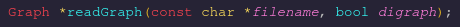
\includegraphics[height=.5cm]{media/readGraph.png}
\end{figure}

prend en argument le nom d'un fichier à lire (qui est supposé d'être dans le format spécifié dans l'énoncé du TP) et une
\texttt{bool} indiquant si le graphe est orienté (vrai) ou pas (faux). En lisant le nombre de sommets, une structure \texttt{Graph} est alloué
et un tableau qui contient des listes d'adjacènes est créé. Le pointeur qui est renvoyé pointe sur un bloc de mémoire nouvellement alloué.
%  Cela est mentionné pour rappeler à
% l'utilisateur

\begin{figure}[h!]
    \centering
    \begin{subfigure}{0.45\textwidth}
        \centering
        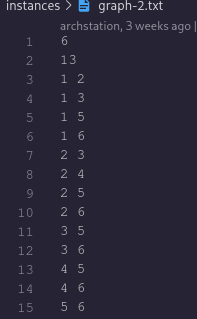
\includegraphics[height=5cm]{media/graph2_txt.png}
        \caption{graph-2.txt}
    \end{subfigure}
    \ding{233}
    \hfill
    \begin{subfigure}{0.45\textwidth}
        \centering
        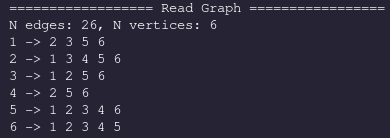
\includegraphics[width=\textwidth]{media/readGraph2.png}
        \caption{\texttt{printGraph(readGraph("graph-2.txt", false))}}
    \end{subfigure}
    \caption{La transformation d'un fichier à un \texttt{Graph} non-orienté.}
    \label{Fig:graph2}

\end{figure}

Un choix d'organisation de la structure se revèle. Pour les graphes non-oriéntés, j'ai décidé que chaque fois que l'on relie
des sommets, je rajoute deux nouvelles arrêts qui vont dans le deux sens. C'est comme si implicitement je rajoutais deux connections orienté.
La justification pour cela c'est quand il s'agit de parcourir un graphe par DFS. Concentrons sur les sommets 1 et 6. Sur ligne 6 de \texttt{graph-2.txt}, on relie
les deux sommets 1 et 6. On voit cet arrêt stocké dans le graphe dans les deux sens; un sens 1 \ding{235} 6 et l'autre sens 6 \ding{235} 1. Imagine si on n'avait pas cette connexion
allant dans le deuxième sens. Si on commence un DFS à partir du sommet 6, on va pas reconnaitre que 1 est adjacent à 6. Cela ne semble pas grave pour cet exemple,
mais il devient clair quand on considère le cas ou 6 est adjacent au sommet 1 et qu'il n'a plus de voisin. Dans ce cas-là un DFS qui démarre de 6 s'arrete immediatement
comme il semble qu'il n'y a plus de chemins. Le cas où le graphe est orienté, on crée un seul arrêt entre les deux sommets dans le sens propre.

\begin{itemize}
    \item [2.] Implémenter une procédure permettant d'exporter au format \texttt{.dot} un graphe donné en argument.
\end{itemize}



La fonction \texttt{createDot} dont la signature :

\newpage
\begin{figure}[h!]
    \centering
    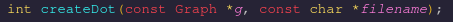
\includegraphics[height=.5cm]{media/createDot.png}
\end{figure}

prend en argument un pointer sur un \texttt{Graph} et qui exporte au format \texttt{.dot} au fichier \texttt{filename} un graphe qui a les mêmes connections
que \texttt{g}. Cette fonction comporte différemment si le graphe est orienté ou pas. Si le graphe est orienté, le stockage des connexions est efficace et il n'y a pas
d'arrêt "rédondant", comme c'est le cas pour les graphes non-orientés. Comme expliqué au-dessus, les graphes non-orientés enregistre des arrêts allant dans les deux
sens pour une seule connexion. Cela nous permet de traverser un \texttt{Graph} peu importe le côté duquel on commencé d'une connexion. Alors, pour créer un fichier
dot qui exporte un graphe non-orienté, on devrait tout d'abord enlever ces arrêtes en rab. On réalise cela avec la fonction \texttt{removeMirrorConnection}.

Après un appel à \texttt{createDot(g, "graph2.dot")}, on contraste l'exportation en dot avec sa représentation interne en Figure \ref{Fig:graph2}.

\begin{figure}[h!]
    \centering
    \begin{subfigure}{0.45\textwidth}
        \centering
        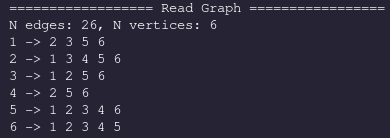
\includegraphics[width=\textwidth]{media/readGraph2.png}
        \caption{graph-2.txt}
    \end{subfigure}
    \hspace{1.25cm}
    \ding{233}
    \hfill
    \begin{subfigure}{0.45\textwidth}
        \centering
        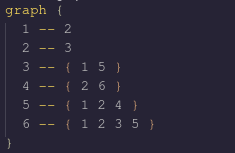
\includegraphics[height=3cm]{media/graph2_dot.png}
        \caption{graph2.dot}
    \end{subfigure}
    \caption{L'exportation en \texttt{dot} d'un \texttt{Graph} non-orienté. L'exportation pour un graphe orienté a tous les arrêts indiquées avec \texttt{$--$} remplacés par \texttt{$->$}}
    \label{Fig:cmp}

\end{figure}

Enfin, on visualise le graphe avec le logiciel \texttt{dot}.

\begin{figure}[h!]
    \centering
    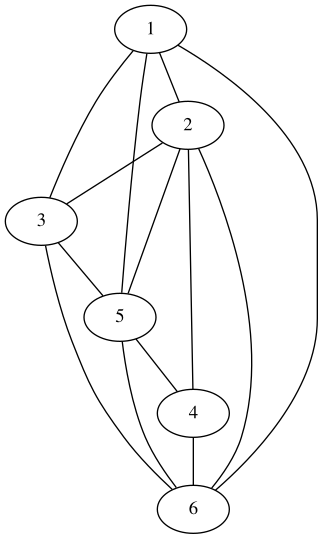
\includegraphics[width=.2\textwidth]{media/graph2.png}
    \caption{\texttt{graph2.dot} en png.}
    \label{Fig:myfig}

\end{figure}

On constate que (contrairement à une version précedente du code qui n'implémentait pas \texttt{removeMirrorConnection}) il n'y a pas d'arrêts
doubles et que le graphe en Figure \ref{Fig:myfig} correspond bien à celui défini par \texttt{graph-2.txt} en Figure \ref{Fig:graph2}


\begin{itemize}
    \item [3.] Implémenter une procédure permettant de visualiser l'arbre dfs d'un graphe donné en entrée.
\end{itemize}

J'ai interpreté les consignes libéralement et j'ai décidé que "visualiser l'arbre dfs" veut dire "afficher à l'écran les sommets que l'on visite
lorsqu'on effecte un parcours dfs". Une autre version du code aurait peut-être exporté un fichier \texttt{.dot} pour chaque pas du parcours. La version du code au moment de rediger ce
rapport ne le fait pas. On peut alors visualiser
un parcours dfs d'un arbre à partir d'un sommet et un graphe donnés en argument à la procédure \texttt{dfsVisualize}.

Si on débarque à partir du sommet 5 du graphe2, on visite les noeuds dans l'ordre suivant:

\begin{figure}[h!]
    \centering
    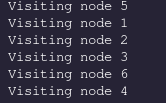
\includegraphics[width=4cm]{media/dfs_vis.png}
    \caption{Visualisation d'un parcours DFS.}
    \label{Fig:viz}
\end{figure}

A partir du sommet 5, on pourrait se déplacer vers les sommets adjacentes: 1, 2, 3, 4, ou 6. Comme le lien entre 5 et 1 a été établit avant les autre connexions,
l'algorithme choisit de visiter le sommet 1. Après avoir visité le sommet 1, on a deux stratégies à considérer. Le premier, le DFS, consiste à continuer à déplacer vers le
enfants du sommet 1, pour continuer en profondeur. L'autre stratégie, le BFS, consiste à visiter les enfants du premier sommet, 5, avant de procéder aux autres descendants. Etant donné
que cela est une implémentation de la stratégie DFS, on visite les enfants de 1 dans un premier temps, voilà donc l'explication pour laquelle on se déplace vers 2, le premier élément
relié avec 1. La stratégie se répète récursivement.

\begin{itemize}
    \item [4.] Implémenter une procédure testant si un graphe est connexe.
\end{itemize}

L'implémentation d'une procédure pour voir si un graphe est connexe ou pas est assez simple à concrétiser. On commence un DFS à n'importe quel sommet
du graphe et on compte le nombre de sommets que l'on visite pour la première fois. A la fin du parcours, si le nombre de sommets visités est égal au nombre de
sommets qui existe dans le graphe, alors on a visité tous les noeuds et le graphe est connexe.

Ce comportement est Implémenté par la fonction \texttt{isConnected} dont la déclaration est:

\begin{figure}[h!]
    \centering
    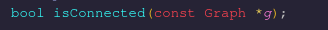
\includegraphics[height=.6cm]{media/isConnected.png}

\end{figure}

\begin{itemize}
    \item [5.] Implémenter une procédure inversant un graphe orienté donné en argument.
\end{itemize}

Afin d'implémenter une procédure inversant un graphe orienté, il faudrait tout simplement créer un autre graphe avec le même nombre de sommets.
En parcourant le graphe originale, on relie les connexions déjà existentes dans l'autre sens. Pour écrire cela en code, on doit considérer la stratégie de
parcourir le graphe. Pour ce faire, on laisse tomber les stratégies singulaire DFS ou BFS et on considère une manière de visiter toutes les connexions du graphe. On pose alors
la stratégie de parcourir le \textit{tableau} des listes d'adjacènces, en inversant toutes les connexions qui existe. On peut imaginer qu'on traverse le graphe verticalement par
rapport à la representation du graphe2 en partie (a) dans Figure \ref{Fig:cmp}. La fonction pertinente est \texttt{reverseGraph}.

Pour plus des détails, veuilleuz consulter le code source en \texttt{cod/src/graph.c} ou regarder la documentation.

\vspace{.5cm}
\noindent \asgold{Partie B :} \aspurp{Composantes fortement connexes}

\begin{itemize}
    \item [1.] Implémenter un algorithme déterminant les composantes fortement connexes d'un graphe orienté.
\end{itemize}

Pour déterminer les composantes fortement connexes, on va se servir de deux parcours DFS. La raison pour laquelle on a implémenté la fonction
\texttt{reverseGraph} c'est parce que le deuxième parcours va s'effecter sur le transpose du graphe dont on veut trouver les composantes fortement connexes. Donc,
muni avec la structure d'une pile déclaré en \texttt{cod/include/stack.h}, on parcours le graphe dans le bon sens, on rajoute à la pile les sommets qui mènent à un
sommet déjà visité ou bien inexistants. Après, on inverse le graphe et en partant du sommet au-dessus de la pile, on effectue encore un DFS pour tomber sur les composantes fortement
connexes. Dans son état actuel, la procédure \texttt{stronglyConnected} crée un nouveau graphe dont les connexions sont des cycles des sommets existants dans la même composantes
fortement connexes. Une visualisation est en ordre.

\begin{figure}[h!]
    \centering
    \begin{subfigure}{0.45\textwidth}
        \centering
        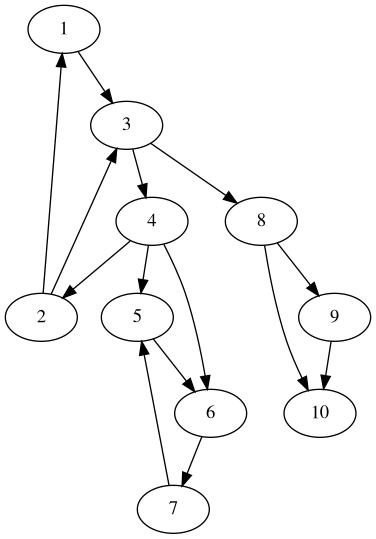
\includegraphics[width=5cm]{media/digraph.png}
        % \caption{Graphe définit en digraph-1.txt}
    \end{subfigure}
    % \hspace{1.25cm}
    \ding{233}
    \hfill
    \begin{subfigure}{0.45\textwidth}
        \centering
        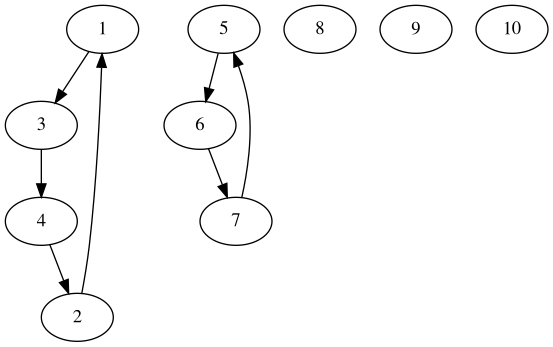
\includegraphics[width=\textwidth]{media/digraph_sg.png}
        % \caption{Les composantes fortement connexes.}
    \end{subfigure}
    \caption{Algorithme qui souligne les composantes fortements connexes. On interprète le graphe à droite pour dire qu'il y a 2 composantes qui sont (pas trivialement) fortements connexes. Une version
    meilleure du code aurait implémenté une procédure qui crée une visualisation qui préserve les connexions originales du graphes, en soulignant les composantes fortement connexes avec des couleurs distinctes.
    Néanmoins, cette routine trouve correctement les composantes fortement connexes: \{1, 2, 3, 4\}, \{5, 6, 7\}, \{8\}, \{9\}, \{10\}.}
    \label{Fig:scc}

\end{figure}


\begin{itemize}
    \item [2.] Analyser la complexité de votre algorithme.
\end{itemize}

Cet algorithme consiste en deux appels à un parcours DFS, ce qui a une complexité de $O(V + E)$. Entretemps l'algorithme utilise une pile dont les actions associé ont une complexité de
$O(V)$. Alors la complexité de cet algorithme est $2*O(V+E) + O(V) \in O(V + E)$

\begin{itemize}
    \item [3.] Implémenter une procédure permettant d'exporter au format \texttt{dot} un graphe donné en argument et indiquant ses composantes fortement connexes.
\end{itemize}

Comme cette fonctionalité a déjà été implémenté implicitement pour la première question, je propose tout simplement la combinaisons des fonctions:
\texttt{createDot(stronglyConnected(g), "graph\_scc.dot");} Cette combinaison marche parce que la fonction \texttt{stronglyConnected} renvoie un graphe dont les connexions sont
qu'entre des composantes fortement connexes. On visualise donc ce graphe avec un appel à la fonction \texttt{createDot} que l'on a vu auparavant. Justement, cette suite de fonctions nous permet
de créer l'image trouvée en Figure \ref{Fig:scc}.

\begin{figure}[h!]
    \centering
    \begin{subfigure}{0.45\textwidth}
        \centering
        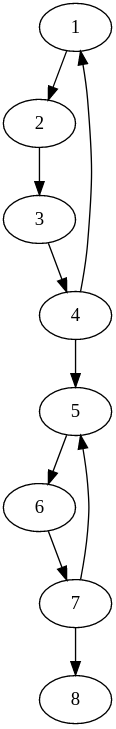
\includegraphics[width=0.25\textwidth]{media/scc.png}
        % \caption{Graphe pour tester la procédure \texttt{stronglyConnected} défini en \texttt{tgraph.c}}
    \end{subfigure}
    % \hspace{1.25cm}
    \ding{233}
    \hfill
    \begin{subfigure}{0.45\textwidth}
        \centering
        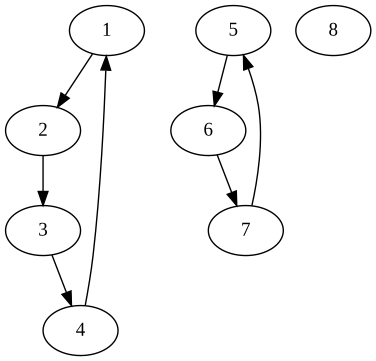
\includegraphics[width=\textwidth]{media/scc_s.png}
        % \caption{Les composantes fortement connexes.}
    \end{subfigure}
    \caption{Application de \texttt{stronglyConnected} avec un autre graphe qui est simple. L'image à droite sougligne les composantes
    fortement connexes du graphe à gauche.}
    \label{Fig:scc2}

\end{figure}

Une version future du code pourra utiliser des couleurs différentes dans la génération d'un fichier \texttt{.dot}
pour distinguer les composantes fortement connexes.

\vspace{.5cm}
\noindent \asgold{Partie C :} \aspurp{Orientation forte d'un graphe}

\begin{itemize}
    \item [1.] Implémenter une procédure testant si un graphe est sans pont. Quelle est sa complexité?
\end{itemize}

Avant dimplémenter une fonction qui détermine si un graphe est sans pont, on devrait écrire une fonction qui détermine déjà si un arrêt individu est
un pont ou pas. Si on enlève l'arrêt concerné d'un graphe et le graphe résultant n'est pas connexe, alors l'arrêt est par définition un pont.  Un graphe entier est donc
sans pont si les arrêts sont tous pas de ponts. Le code s'écrit aisement, on parcours tous les arrêts et si il y a un seul entre eux qui soit un pont,
notre fonction \texttt{hasBridge} renvoie vrai.

Pour déterminer sa complexité on considère le fait qu'on devrait verifier si \textit{chaque} arrêt est un pont. Donc, on devrait appeler la fonction
\texttt{isBridge} $E$ fois. La fonction \texttt{isBridge} teste si un arrêt est un pont en quittant la connexion et vérifiant si le graphe qui en résulte est connexe
ou pas. Finalement, la procédure pour déterminer si un graphe est connexe ou pas consiste d'un seul parcours DFS. On conclut alors que \texttt{isBridge} consiste d'un parcours
DFS et donc est de class de complexité $O(V + E)$, et que la procédure \texttt{hasBridge} consiste de $E$ appels d'une procédure de complexité $O(V + E)$. Alors, la complexité
de la procédure testant si un graphe est sans pont est $O(E(V + E))$.

\begin{itemize}
    \item [2.] Démontrer qu'un graphe $G$ est fortement orientable si et seulement si $G$ ne possède pas de pont.
\end{itemize}

Pour démontrer cela, on suppose que G est fortement orientable. Par définition, cela veut dire qu'il existe une orientation fortement connexe de $G$. De plus, cela implique
que pour deux sommets quelconque $u$ et $v$, il existe un chemin de $u$ vers $v$ et un chemin de $v$ vers $u$. Si on imagine le scénario où on enlève
n'importe quel arc du graphe $G$, on peut - au pire - casser l'un des chemins entre $u$ et $v$. Vu qu'un arc a une et seulement une orientation, il est impossible que le chemin en avance
$u$ \ding{235} $v$ et le chemin $v$ \ding{235} $u$ en revers traverse l'arrêt qu'on va enlever. Autrement dit, comme un arc a un seul sens, si on enlève un arc quelconque on aura \textbf{toujours} un graphe
qui reste quand même \textit{connexe}, mais pas forcémment \textit{fortement connexe}. Par conséquence, $G$ ne contient pas de pont et on a démontré l'égalité dans la direction en avant.

Pour attaquer la deuxième direction, on suppose que $G$ ne possède pas de pont. Alors, on peut toujours supprimer un arrêt du $G$ sans le priver d'être connexe. Il existe alors une orientation telle que
pour deux sommets quelconque $u$ et $v$, il existe un chemin de $u$ vers $v$ ou un chemin de $v$ vers $u$. Cela est une conséquence immédiate de la connectivité du graphe. Pour vérifier un orientation forte, on
doit garantir qu'il existe un chemin dans les deux sens! Comme il n'y a aucun pont, il y a toujours un arc "en extra" pour aller dans l'autre sens et compléter le cycle d'un graphe.

On a donc vérifié l'égalité dans les deux sens.

\begin{itemize}
    \item [3.] Implémenter une procédure déterminant une orientation forte d'un graphe non orienté sans pont. Analyser sa complexité.
\end{itemize}

    Une version future du code qui sera mise à jour sur github implémentera cette routine.

\begin{itemize}
    \item[4.] Exécuter l'algorithme
\end{itemize}

    Une version future du code qui sera mise à jour sur github testera cette procédure.

\vspace{.5cm}
\noindent \asgold{Remarques :} \aspurp{Repo github}

Une version minimale du répertoire sera inclu dans le zip à rendre sur moodle. Pour voir le répertoire complet et mis à jour, consultez le
github. Les procédures basiques qui sont utilisées dans ce TP sont testées au moment de la construction avec le logiciel \texttt{CTest} et \texttt{CMake}. Si jamais cela vous intéresse,
vous pouvez construire le projet en suivant les instructions sur le \texttt{README.md} du projet. De la documentation technique a été générée par \texttt{Doxygen} et de la
documentation du projet qui est plus générale et qui contient des exemples pour montrer l'API a été construite avec \texttt{Mkdocs} et hébergé par \texttt{readthedocs}.


% \newpage
\end{document}